\section{3-Way Join}
Building on the correlation analysis between course grades and benchmarks for CSC1015F, additional information concerning each student's Sakai usage is taken into account. Along with the ``Grades.CSV'' and ``Benchmarks.CSV'' files, a 3rd CSV ``Events.CSV'' is loaded into CouchDB via the nETL application. Since a single student may be associated with many rows in the Event data (sometimes even thousands of rows), a reduce function is used within the MapReduce job to aggregate the Events rows into a single document that is a count of Sakai presence events for first and second semester, with the output of this aggregation (and also the documents for the Grade and Benchmark entities) saved as a view, again, sorted by StudentID. Similarly to the 2-Way analysis of CSC1015F Grade/Benchmarks correlation, a CouchDB List function is used for retrieving data from the view index and performing the 3-way join.

In other words, this analysis addresses the question of whether making more frequent use of the Sakai platform is shown to increase course performance for CSC1015F, as well as looking at the correlation between benchmarking scores and LMS usage. However, the Events cannot be associated with particular courses for the purposes of this study since the Events data FK to course ID, is strictly relevant to the Sakai system only; the grades data has not been exported directly from the Sakai platform and the id that is referenced by Sakai events is not present in the dataset used. As such, this analysis takes into account only ``general usage'' of the Sakai LMS, and not usage of Sakai for these particular courses.

\subsection{nETL Configuration}
nETL Tasks 1 and 2 are the same as run previously for the 2-Way join, except that only course grades from 2016 are used (since the Events exports is only from 2016). The 3-Way join introduces a 3rd task - Task 5 - in which lines from the ``Events.CSV'' file are extracted, transformed and loaded into CouchDB using the nETL application. Tasks 3, 4 \& 5 as JSON configuration files are included in the appendix at \ref{netl-tasks-3-4-5-config}.

Using nETL, Task 5 execution comprises an iterative extraction of 30 000 lines at a time. Each line from each batch undergoes a series of transformations before the entire batch is loaded into CoucDB via the \textit{\_bulk\_docs} endpoint, following which, the iterative extraction continues. A list of the transformations applied to each line extract from the ``Events.CSV'' file by nETL is shown below:

\subsubsection{Task 5 Transformations (Events)}
\begin{enumerate}
  \item A line is converted into a JavaScript object (which relates directly to the JSON format of CouchDB documents) with the fields:
        \begin{itemize}
          \item event\_date
          \item event\_id
          \item uct\_id
          \item site\_key
          \item ref
        \end{itemize}
  \item Lines are filtered on the ``uct\_id'' and ``event\_id'' fields; only events with an event type of ``presence'' (event\_id = 282) for students enrolled in CSC1015F in 2016 are considered.
  \item An attribute (``type\_'') is then added to each line (that weren't removed in filtering step), and given the value ``event'' to identify each object as a line of the Event entity type.
  \item Line attributes are whitelisted. The resultant lines each have the the following attributes:
        \begin{itemize}
          \item type\_
          \item event\_date
          \item event\_id
          \item uct\_id
          \item site\_key
        \end{itemize}
\end{enumerate}

\subsection{MapReduce Functions}
The map function for this analysis is included in the appendix (see \ref{3-way-join-map-function}). Each document passed to the map function is treated according to the logic shown in the activity diagram in Figure \ref{fig-3-way-join-map-function}. Logical handling of the Grade and Benchmark entities is discussed previously.If the document is a line of the Events entity then the date of the event is categorized as either having occurred in semester 1 or semester 2. A key of [Student ID, 0, Year] is emitted along with the value (a 2-index tuple) of [S1, S2]. The S1, and S2 variables are 0 by default, and depending on the date of the presence event, one of these variables is altered to be `1'.

Using the \_sum reduce function, an aggregation is done across all documents with the same key; this means that per a student, an aggregation is performed on a single Grade document, a single Benchmark document, and many Events documents in which the S1 and S2 variables are summed to form the tuple [sum of S1, sum of S2]. Because of the key output of each type of entity, the resulting view-index is ordered by StudentID; for each StudentID documents are ordered by the second index in the key output (course), which means that Benchmarks and Events entities are sorted to be before grades for a student; and sorting via the 3rd index of each key results in benchmark data always being sorted to be before Events documents. As such, during view-index retrieval it can be taken as given that for a single student ID, first documents of type Benchmark will be retrieved, followed by documents of type Event, followed by documents of type Grade.

\begin{figure}[ht]
    \centering
    \begin{mdframed}
        \centering
        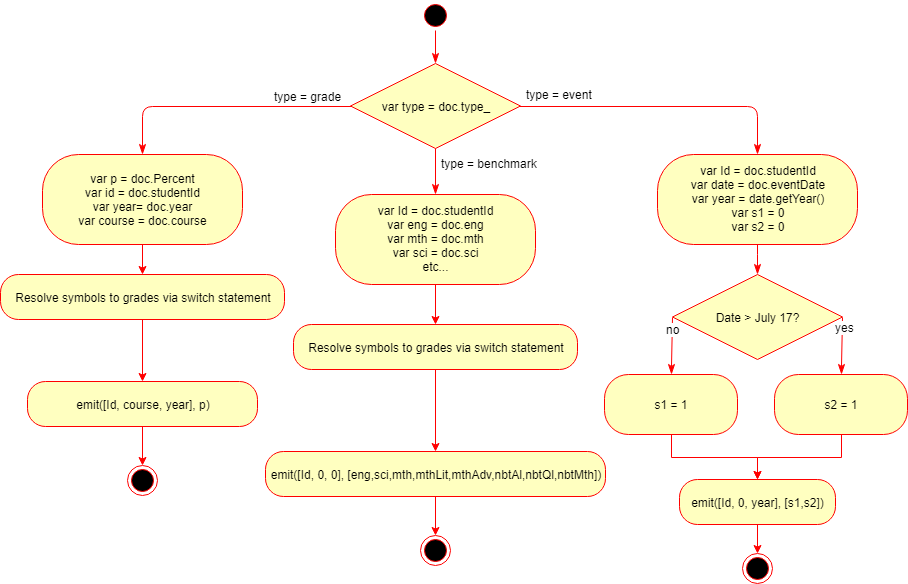
\includegraphics[scale=0.35]{./resources/figures/3-way-join-map.png}
    \end{mdframed}
    \caption[2-Way Join Map Function]{\textbf{Figure \ref{fig-3-way-join-map-function}: Map function logic required for the 2-way join.} This logic is applied to every document during index calculation (excluding documents with an \_id of ``\_design/*''). The logic used to normalize grades-as-symbols to percentages is shown in Table \ref{tbl-grades-normalize} for the Grades data, and \ref{tbl-benchmarks-normalize} for the Benchmarks data.}
    \label{fig-3-way-join-map-function}
\end{figure}

\subsection{List Function}
The List function is invoked via an HTTP request to the URI: \texttt{https://localhost:5984/msc /\_design/3-way-join/\_list/3-way-join-list/3-way-join-view?reduce=true}. On execution the list function executes the ``provides'' function, in which output type of ``CSV'' (plain text) is specified as as download file. List function logic as shown in Figure \ref{fig-3-way-join-list-function} is executed in the callback passed as a parameter to the ``provides'' function.

On initial invocation and within the body of the callback, the variables `currentStudent', `currentYear', and `currentLine' are set to null. Following this an iteration over the index is initiated within a while loop with the loop invariant the result of a call to the ``getRow'' function. While the loop invariant remains true (i.e. so long as the ``getRow'' function returns a row and not `false', which occurs after the last row has been retrieved from the index), a row - a reduced result - is processed (in the URI the parameter ``reduce'' is set to true, so ONLY reduced output is retrieved from the view). Similarly to List function logic for the 2-way join, after the loop invariant becomes false the last line is still in memory and is sent if necessary.

For every result retrieved from the reduce output , the StudentID of the row being processed is checked and compared to the StudentID of the previous row. If the current StudentID is not the same as the previous StudentID, a line of the CSV is emitted before the row is processed. Then, the type of result being processed is checked (either the document is of type ``benchmark'', ``event'' or ``grade''), and depending on the type different values are stored in a variable called ``currentLine''. For every StudentID, all types of documents are processed in turn (first the benchmark documents, then the event documents, then the grade documents) before being emitted. This allows the join to be performed via sequentially adding to the ``currentLine'' variable for a single student.

As as result of the MapReduce function, for every StudentID, exactly one ``benchmark'' result and one ``event'' document is processed. But a student can have several ``grade'' documents if the course was repeated in subsequent years. To catch this case, when processing documents of type ``grade'' within the switch statement, a further check is done to see if the attribute `year' of the current row has already been processed and is different from a preceding row. If so, the ``currentLine'' is emitted and the fields relating to grade documents are reset, and then repopulated with values from the current row (``currentLine'' itself is not reset). For every Event row processed both the first and second semester event count are exported to the CSV despite that only the first semester events are used, since there is negligible performance cost in terms of processing time or storage space and so there is little incentive to discard good data.

Conceptually, sending ``currentLine'' involves a call to a helper function provided within the execution context of CouchDB List functions - the ``send'' function. This function is wrapped within a subroutine (a function nested within the callback) that first checks that the currentLine variable contains data from the Grades and Benchmarks and Events entity, and then sends a comma-delimited string along a stay-alive network request - this is handled automatically by the HTTP client, which in the case of this project is simply the Google Chrome browser. From a user's perspective, it appears that a file is simply being downloaded; the rate at which the file downloads is equal to the rate at which the loop data is output by the send function. The download completes on completion of the List function. Code for the loop function is included in the appendix at \ref{3-way-join-list-function}.

\begin{figure}[H]
    \centering
    \begin{mdframed}
        \centering
        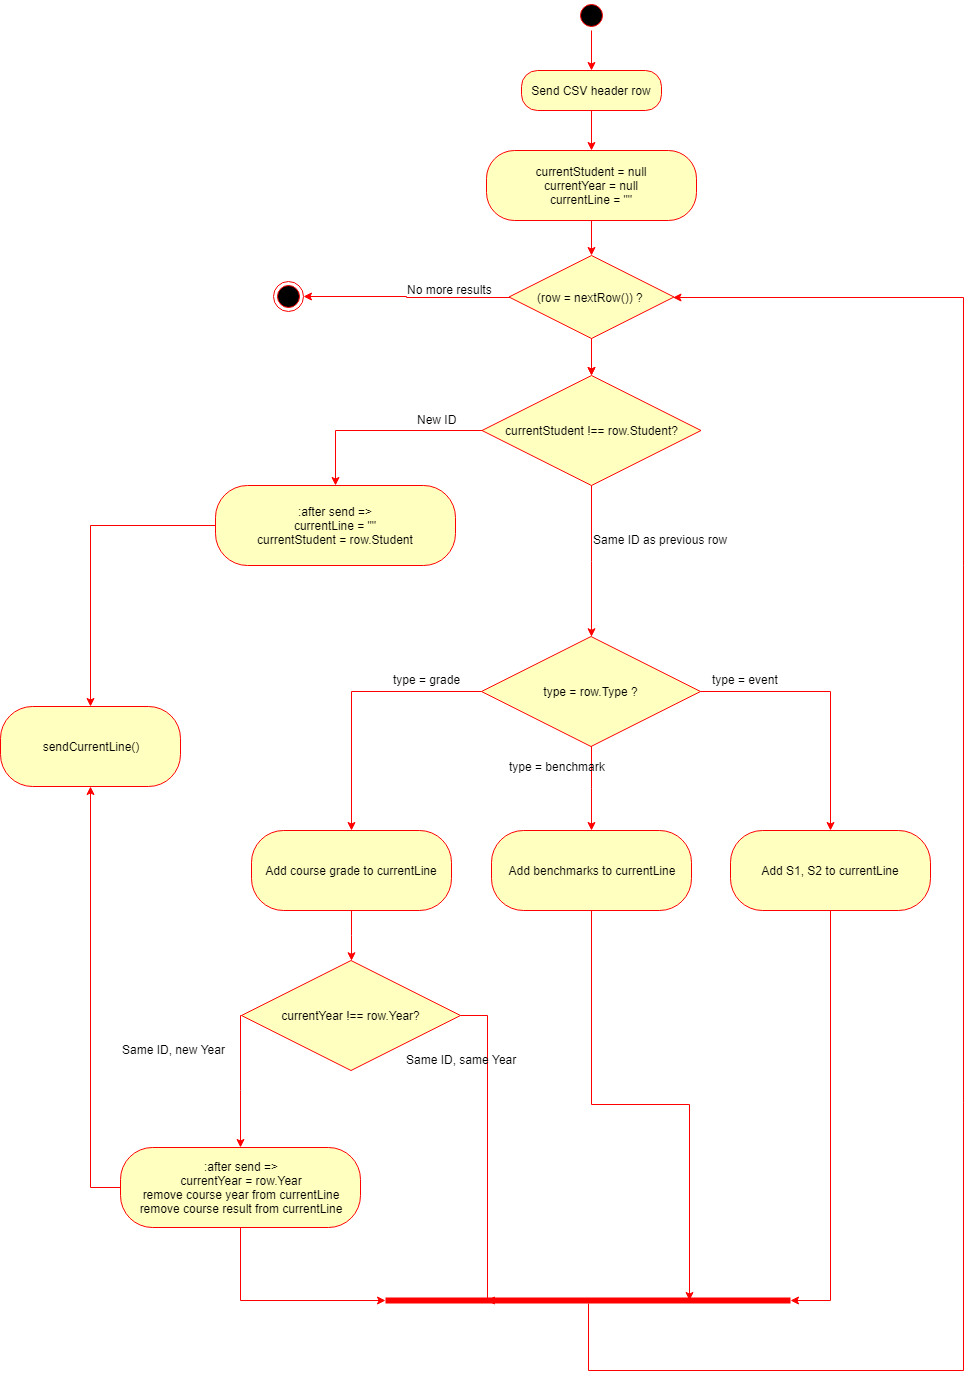
\includegraphics[scale=0.35]{./resources/figures/3-way-join-list.png}
    \end{mdframed}
    \caption[3-Way Join List Function]{\textbf{Figure \ref{fig-3-way-join-list-function}: List function logic required to join the Grades, Benchmarks and Events entities.} Activity diagram of the code executed within the callback passed to the provides function executed by CouchDB during runtime of List function.}
    \label{fig-3-way-join-list-function}
\end{figure}

\subsection{Output}
A sample of the resultant joined dataset is shown in Figure \ref{fig-3-way-csv-output}
\begin{figure}[H]
    \centering
    \begin{mdframed}[rightline=false,leftline=false]
        \centering
        \begin{BVerbatim}[fontsize=\tiny]

+------+---------+----------+-------+----------+----------+----------+--------------+--------------+--------+--------+---------+------+------+
| Year |   ID    |  Course  | Grade | Gr12 Eng | Gr12 Sci | Gr12 Mth | Gr12 Mth Lit | Gr12 Mth Adv | NBT AL | NBT QL | NBT Mth |  S1  |  S2  |
+------+---------+----------+-------+----------+----------+----------+--------------+--------------+--------+--------+---------+------+------+
| 2016 | 2862568 | CSC1015F |    63 |       80 |        0 |       95 |            0 |            0 |     78 |     79 |      82 |  330 |  138 |
| 2016 | 2864266 | CSC1015F |    64 |       55 |        0 |       74 |            0 |            0 |     59 |     66 |      61 |  557 |  620 |
| 2016 | 2924430 | CSC1015F |    56 |       69 |       94 |       96 |            0 |            0 |     49 |     64 |      77 |  550 |  306 |
| 2016 | 2925212 | CSC1015F |    60 |       76 |        0 |       77 |            0 |            0 |     69 |     84 |      73 |  124 |  155 |
| 2016 | 2928032 | CSC1015F |    30 |       76 |        0 |       73 |            0 |            0 |     85 |     53 |      35 |  307 |  296 |
| 2016 | 2930116 | CSC1015F |    91 |       89 |       91 |       93 |            0 |            0 |     81 |     94 |      94 |  228 |  188 |
| 2016 | 2932174 | CSC1015F |    65 |       79 |        0 |       80 |            0 |            0 |     50 |     64 |      55 |  220 |  225 |
| 2016 | 2932204 | CSC1015F |    30 |       79 |        0 |       84 |            0 |            0 |     66 |     59 |      71 |   78 |    2 |
| 2016 | 2934500 | CSC1015F |    61 |       85 |        0 |       87 |            0 |            0 |     63 |     65 |      78 | 1054 | 1019 |
| 2016 | 2941940 | CSC1015F |    48 |       69 |        0 |       76 |            0 |            0 |     71 |     68 |      69 |  556 |  725 |
| 2016 | 2943800 | CSC1015F |    58 |       67 |        0 |       79 |            0 |            0 |     72 |     65 |      77 |  463 |  531 |
| 2016 | 2944396 | CSC1015F |    61 |       87 |        0 |       82 |            0 |            0 |     69 |     76 |      84 |  935 | 1252 |
| 2016 | 2944854 | CSC1015F |    67 |       82 |        0 |       92 |            0 |            0 |     74 |     83 |      79 |  336 |  264 |
| 2016 | 2946538 | CSC1015F |    48 |       77 |        0 |       74 |            0 |            0 |     77 |     64 |      56 |  533 |  242 |
| 2016 | 2950404 | CSC1015F |    89 |       80 |       75 |       91 |            0 |            0 |     83 |     74 |      85 |  164 |   93 |
| 2016 | 2951308 | CSC1015F |    30 |       80 |        0 |       71 |            0 |            0 |     70 |     62 |      54 |  130 |   50 |
| 2016 | 2951954 | CSC1015F |    42 |        0 |        0 |        0 |            0 |            0 |     78 |     86 |      57 |  309 |   58 |
+------+---------+----------+-------+----------+----------+----------+--------------+--------------+--------+--------+---------+------+------+

        \end{BVerbatim}
    \end{mdframed}
    \caption[Sample of 3-way CSV output]{\textbf{Figure \ref{fig-3-way-csv-output}: Sample of the 3-way join output CSV.} List function output is a CSV download with the schema as represented in this figure. The full CSV has 586 rows (including a header row). Since only a single year of data was analyzed, there are no repeated StudentIDs in the dataset.}
    \label{fig-3-way-csv-output}
\end{figure}
